\documentclass[12pt]{article}
\usepackage[utf8]{inputenc}
\usepackage{geometry}
\geometry{letterpaper, margin=0.25in}
\usepackage{graphicx} 
\usepackage{parskip}
\usepackage{booktabs}
\usepackage{array} 
\usepackage{paralist} 
\usepackage{verbatim}
\usepackage{subfig}
\usepackage{fancyhdr}
\usepackage{sectsty}
\usepackage[shortlabels]{enumitem}

\pagestyle{fancy}
\renewcommand{\headrulewidth}{0pt} 
\lhead{}\chead{}\rhead{}
\lfoot{}\cfoot{\thepage}\rfoot{}

%%% ToC (table of contents) APPEARANCE
\usepackage[nottoc,notlof,notlot]{tocbibind} 
\usepackage[titles,subfigure]{tocloft}
\renewcommand{\cftsecfont}{\rmfamily\mdseries\upshape}
\renewcommand{\cftsecpagefont}{\rmfamily\mdseries\upshape} %

\usepackage{amsmath}
\usepackage{amssymb}
\usepackage{mathtools}
\usepackage{empheq}
\usepackage{xcolor}
\usepackage{bbm}
\usepackage{tikz}
\usepackage{pgfplots}
\usepackage{tikz-cd}
\pgfplotsset{compat=1.18}
\usetikzlibrary{intersections, decorations.markings}
\usepgfplotslibrary{fillbetween}
\tikzset{
    marking along/.style n args={2}{
        decoration={
                markings, 
                mark=at position #1 with {\arrow{#2}}
        },
        postaction={decorate}
        },
    marking along/.default={0.5}{>}
}

\newcommand{\ans}[1]{\boxed{\text{#1}}}
\newcommand{\vecs}[1]{\langle #1\rangle}
\renewcommand{\hat}[1]{\widehat{#1}}

\renewcommand{\P}{\mathbb{P}}
\newcommand{\R}{\mathbb{R}}
\newcommand{\E}{\mathbb{E}}
\newcommand{\Z}{\mathbb{Z}}
\newcommand{\N}{\mathbb{N}}
\newcommand{\Q}{\mathbb{Q}}
\newcommand{\C}{\mathbb{C}}

\newcommand{\ind}{\mathbbm{1}}
\newcommand{\qed}{\quad \blacksquare}

\newcommand{\brak}[1]{\left\langle #1 \right\rangle}
\newcommand{\bra}[1]{\left\langle #1 \right\vert}
\newcommand{\ket}[1]{\left\vert #1 \right\rangle}

\newcommand{\abs}[1]{\left\vert #1 \right\vert}
\newcommand{\mfX}{\mathfrak{X}}
\newcommand{\ep}{\varepsilon}

\newcommand{\Ec}{\mathcal{E}}
\newcommand{\Nc}{\mathcal{N}}
\newcommand{\A}{\mathcal{A}}
\newcommand{\F}{\mathcal{F}}
\newcommand{\Cc}{\mathcal{C}}
\newcommand{\B}{\mathcal{B}}
\newcommand{\M}{\mathcal{M}}
\newcommand{\X}{\chi}
\renewcommand{\L}{\mathcal{L}}

\newcommand{\sub}{\subseteq}
\newcommand{\st}{\text{ s.t. }}
\newcommand{\card}{\text{card }}
\renewcommand{\div}{\vspace*{10pt}\hrule\vspace*{10pt}}
\newcommand{\surj}{\twoheadrightarrow}
\newcommand{\inj}{\hookrightarrow}
\newcommand{\biject}{\hookrightarrow \hspace{-8pt} \rightarrow}
\renewcommand{\bar}[1]{\overline{#1}}
\newcommand{\overcirc}[1]{\overset{\circ}{#1}}
\newcommand{\diam}{\text{diam }}
\newcommand{\iid}{\overset{	ext{iid}}{\sim}}

\renewcommand{\Re}{\text{Re}\,}
\renewcommand{\Im}{\text{Im}\,}
\newcommand{\Var}{\text{Var}\,}
\newcommand{\Cov}{\text{Cov}\,}
\newcommand{\tr}{\text{tr}\,}


\DeclareMathOperator*{\argmax}{\arg\max}
\DeclareMathOperator*{\argmin}{\arg\min}

\newcommand{\sign}{\text{sign}\,}

\newcommand*{\tbf}[1]{\ifmmode\mathbf{#1}\else\textbf{#1}\fi}

\usepackage{tcolorbox}
\tcbuselibrary{breakable, skins}
\tcbset{enhanced}
\newenvironment*{tbox}[2][gray]{
    \begin{tcolorbox}[
        parbox=false,
        colback=#1!5!white,
        colframe=#1!75!black,
        breakable,
        title={#2}
    ]}
    {\end{tcolorbox}}

\newenvironment*{exercise}[1][red]{
    \begin{tcolorbox}[
        parbox=false,
        colback=#1!5!white,
        colframe=#1!75!black,
        breakable
    ]}
    {\end{tcolorbox}}

\newenvironment*{proof}[1][blue]{
\begin{tcolorbox}[
    parbox=false,
    colback=#1!5!white,
    colframe=#1!75!black,
    breakable
]}
{\end{tcolorbox}}
\newenvironment*{proposition}[1][gray]{
    \begin{tcolorbox}[
        parbox=false,
        colback=#1!5!white,
        colframe=#1!75!black,
        breakable
    ]}
    {\end{tcolorbox}}

\title{APMA 1360 - Homework 7}
\author{Milan Capoor}
\date{21 March 2025}

\begin{document}
\maketitle


\section{Brusselator model}

Consider the system
\[
    \dot{x} = 1 - (b+1) x + a x^2 y, \qquad
    \dot{y} = b x - a x^2 y,
\]
which is a model for autocatalytic chemical reactions, where $x,y\geq0$ and $a,b>0$.
\begin{enumerate}[(i)]
    \item Find all equilibria and use the Jacobian to classify them.

          \color{blue}
          \[\begin{array}{rl}
                  0 & = 1 - (b+1)x + ax^2y \\
                  0 & = b x - a x^2 y      \\ \hline
                  0 & = 1 - x
              \end{array}\]

          Substituting $x = 1$,
          \[0 = b - ay \implies y = \frac{b}{a}\]
          so our only equilibrium is $\boxed{(1, b/a)}$. The Jacobian is
          \[J(x, y) = \begin{pmatrix}
                  -b-1 + 2axy & ax^2  \\
                  b - 2axy    & -ax^2
              \end{pmatrix} \implies J(1, b/a) = \begin{pmatrix}
                  -b -1 + 2b & a  \\
                  b - 2b     & -a
              \end{pmatrix} = \begin{pmatrix}
                  b - 1 & a  \\
                  -b    & -a
              \end{pmatrix}\]


          We know
          \begin{align*}
              \lambda_1 \lambda_2   & = -ab + a + ab = a \\
              \lambda_1 + \lambda_2 & = b-1 - a
          \end{align*}

          Since $a > 0$, $\det J > 0$ and we know there cannot be a saddle. $\tr J = b - a - 1$ is
          \[\begin{cases}
                  > 0 & \text{if } b-a > 1  \\
                  < 0 & \text{if } b- a < 1
              \end{cases} \implies \boxed{\begin{cases}
                      \text{repeller if } b-a > 1 \\
                      \text{attractor if } b-a < 1
                  \end{cases}}\]

          \color{black}

    \item Show that a Hopf bifurcation occurs at some value of the parameter $b$ (this value will depend on $a$).

          \color{blue}
          Let
          \[F(x, y) = \begin{pmatrix}
                  1 - (b+1)x + ax^2y \\
                  b x - a x^2 y
              \end{pmatrix}\]
          Clearly $F \in C^3$.

          In part i, we showed that the Jacobian at the equilibrium is
          \[J(1, b/a) = \begin{pmatrix}
                  b-1 & a  \\
                  -b  & -a
              \end{pmatrix}\]

          Notice that we could manually calculate the eigenvalues by
          \begin{align*}
              0       & = (b - 1 - \lambda)(-a - \lambda) + ab                 \\
                      & = \lambda^2 + (a - b + 1)\lambda + a                   \\
              \lambda & = \frac{-(a - b + 1) \pm \sqrt{(a - b + 1)^2 - 4a}}{2} \\
              \lambda & = \alpha(a, b) \pm i \beta(a, b)
          \end{align*}

          In order for a Hopf Bifurcation to occur, we need
          \begin{enumerate}
              \item $\alpha(a, b) = 0$
              \item $\beta(a, b) \neq 0$
              \item $\frac{\partial \alpha}{\partial a} \neq 0$
              \item $\frac{\partial \alpha}{\partial b} \neq 0$
          \end{enumerate}

          This gives us a system of equations
          \begin{align}
              -(a - b + 1)                                      & = 0    \\
              (a - b+1)^2 - 4a                                  & \neq 0 \\
              \frac{\partial \alpha}{\partial a} = -\frac{1}{2} & \neq 0 \\
              \frac{\partial \alpha}{\partial b} = 1            & \neq 0
          \end{align}

          Equation (1) implies $b = a+1$. Substituting this into (2) gives
          \[(a - (a + 1) + 1)^2 - 4a = -4a < 0\]
          and equations (3) and (4) are trivially satisfied.

          Hence, for $\boxed{b = a + 1}$, a Hopf Bifurcation occurs around the equilibrium $(1, 1+1/a)$.


          \color{black}

    \item Find the approximate period of the periodic orbit that bifurcates from the equilibrium at this Hopf bifurcation.

          \color{blue}
          We know that the period of the periodic orbit is given by $\approx \frac{2\pi}{\beta(a, b)}$. Letting, $b = a + 1$,
          \[\lambda^2 + (a - b + 1)\lambda + a = 0 \implies \lambda^2 + a = 0 \implies \lambda = \pm i \sqrt{a} \implies \beta(a, b) = \sqrt{a}\]
          so the period is given by
          \[\boxed{\approx \frac{2\pi}{\sqrt a}}\]

          \color{black}
\end{enumerate}

\pagebreak

%%%%%%%%%%%%%%%%%%%%%%%%%%%%%%%%

\section{Bead on a rotating hoop revisited}

Consider the second-order equation
\begin{equation}\label{e1}
    \frac{d^2\phi}{d t^2} = - a \frac{d\phi}{d t} + (\gamma\cos\phi-1) \sin\phi
\end{equation}
that we discussed as a model for a bead that slides on a rotating hoop subject to gravitational and friction forces. The parameter $a$ and $\gamma$ are both strictly larger than zero: we keep $a>0$ fixed and vary $\gamma>0$.
\begin{enumerate}[(i)]
    \item Define the angular velocity $v:=d\phi/d t$ and write (\ref{e1}) as a first-order system, which we refer to as equation (2), for the variables $(\phi,v)$.

          \color{blue}
          Let $v = d\phi/dt$. Then, we have
          \[\begin{cases}
                  \dot \phi = v \\
                  \dot v = -av + (\gamma\cos\phi - 1)\sin\phi
              \end{cases}\]

          \color{black}

    \item Find the equilibria of the system (2) and determine their stability properties. Also, identify all bifurcations in this system.

          \color{blue}
          We want $(\dot \phi, \dot v) = (0, 0)$ which immediately suggests $v = 0$, so
          \[(\gamma \cos \phi - 1) \sin \phi = 0 \implies \begin{cases}
                  \cos \phi = 1/\gamma \\
                  \sin \phi = 0
              \end{cases} \implies \phi = \{\arccos \frac{1}{\gamma}, 0, \pi\}\]
          where $\gamma \geq 1$ (else $\cos \phi = 1/\gamma$ has no solutions).

          We have Jacobian
          \begin{align*}
              J(\phi, v)                     & = \begin{pmatrix}
                                                     0                             & 1  \\
                                                     \gamma \cos 2\phi - \cos \phi & -a
                                                 \end{pmatrix} \\
              J(\arccos \frac{1}{\gamma}, 0) & = \begin{pmatrix}
                                                     0                    & 1  \\
                                                     2 - \frac{1}{\gamma} & -a
                                                 \end{pmatrix}          \\
              J(\pi, 0)                      & = \begin{pmatrix}
                                                     0          & 1  \\
                                                     \gamma + 1 & -a
                                                 \end{pmatrix}                    \\
              J(0, 0)                        & = \begin{pmatrix}
                                                     0          & 1  \\
                                                     \gamma - 1 & -a
                                                 \end{pmatrix}
          \end{align*}

          Further,
          \[\det J(\arccos \frac{1}{\gamma}, 0)  = 2 - \frac{1}{\gamma} > 0 \quad \forall \gamma\]
          hence we have ad an attractor or repeller. We can check
          \[\tr J(\arccos \frac{1}{\gamma}, 0) = -a < 0 \quad \forall a > 0\]
          which means that $\boxed{\phi = \arccos \frac{1}{\gamma}\text{ is an attractor}}$

          Similarly,
          \[\det J(\pi, 0) = -(\gamma + 1) < 0 \quad \forall \gamma\]
          so $\boxed{\phi = \pi\text{ is a saddle for all }\gamma}$

          Finally,
          \[\det J(0, 0) = -(\gamma - 1)\]
          is
          \[\begin{cases}
                  < 0 & \text{if } \gamma > 1 \\
                  > 0 & \text{if } \gamma < 1
              \end{cases}\]
          and
          \[\tr J(0, 0) = -a < 0 \quad \forall \gamma\]
          so $\boxed{\phi = 0\text{ is a saddle for } \gamma > 1\text{ and an attractor } \gamma < 1 }$

          \begin{center}
              \color{black}
              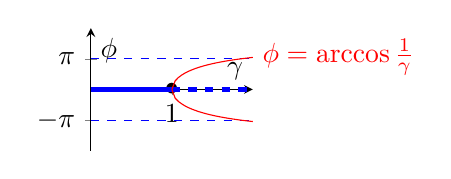
\begin{tikzpicture}
                  \begin{axis}[
                          width=0.3\textwidth,
                          axis lines=middle,
                          no markers,
                          xtick={1},
                          ytick={-1, 0, 1},
                          yticklabels={$-\pi$, $0$, $\pi$},
                          clip=false,
                          xlabel={$\gamma$},
                          ylabel={$\phi$},
                          domain=-2:2,
                          ymin=-2, ymax=2,
                          xmin= 0, xmax=2,
                          view = {0}{90}
                      ]

                      \node at (1, 0) {$\bullet$};

                      \addplot[blue, ultra thick, domain=0:1] {0};
                      \addplot[blue, ultra thick, dashed, domain=1:2] {0};

                      \addplot[blue, dashed, domain=0:2] {1};
                      \addplot[blue, dashed, domain=0:2] {-1};

                      \addplot[red, domain=1:2] {pi/180*acos(1/x)} node[right] {$\phi = \arccos \frac{1}{\gamma}$};
                      \addplot[red, domain=1:2] {-pi/180*acos(1/x)};
                  \end{axis}
              \end{tikzpicture}
          \end{center}

          Clearly, we have a $\boxed{\text{supercritical pitchfork bifurcation}}$ at $\gamma = 1$.
          \color{black}

    \item Compare your findings to those we obtained for the one-dimensional system where we omitted the second-order derivative $d^2\phi/d t^2$.

          \color{blue}

          In the case where we omitted the second-order derivative, we had equilibria at $\phi = 0, \pi$, with
          \begin{itemize}
              \item $\phi = 0$ stable if $\gamma < 1$ and unstable if $\gamma > 1$
              \item $\phi = \pi$ is always unstable
          \end{itemize}
          and a pitchfork bifurcation at $\gamma =1$.

          In the case where we included the second-order derivative, we again have a pitchfork bifurcation at $\gamma = 1$, but now
          \begin{itemize}
              \item $\phi = 0$ is an attractor for $\gamma < 1$ and a saddle for $\gamma > 1$
              \item $\phi = \pi$ is a saddle
              \item $\phi = \arccos \frac{1}{\gamma}$ is an attractor
          \end{itemize}

          And this makes sense! In a sense, this is exactly the same result but in the higher dimension, we have saddles instead of unstable equilibria.

\end{enumerate}

%%%%%%%%%%%%%%%%%%%%%%%%%%%%%%%%

\end{document}